%!TEX program=xelatex
\documentclass{beamer}
\usetheme{focus}
% Full instructions available at:
% https://github.com/elauksap/focus-beamertheme

\usepackage{ctex}

\usepackage{listings}
\usepackage{golang}
\usepackage{xcolor}

\title{Go并发元件}
%\subtitle{Subtitle}
\author{黎相敏}
\titlegraphic{
\includegraphics[scale=1.25]{focuslogo.pdf}}
\institute{上海观源信息科技有限公司 \\ 上海市闵行区紫竹科技园4号楼303B}
\date{12/01/2019}

\lstset{ % add your own preferences
    frame=trBL, %single,
    basicstyle=\ttfamily\footnotesize,
    keywordstyle=\color{red},
    numbers=left,
    numbersep=8pt,
    showstringspaces=false, 
    stringstyle=\color{blue},
    tabsize=2,
    language=golang % this is it !
}
\renewcommand{\lstlistingname}{代码片段}% Listing -> 代码片段

% command macros to save typing
\newcommand{\WaitGroup}{\texttt{WaitGroup}}
\newcommand{\Mutex}{\texttt{Mutex}}
\newcommand{\RWMutex}{\texttt{RWMutex}}
\newcommand{\Cond}{\texttt{Cond}}
\newcommand{\Once}{\texttt{Once}}
\newcommand{\Pool}{\texttt{Pool}}

\begin{document}

    \begin{frame}
        \maketitle
    \end{frame}

    \begin{frame}{大纲}
        \tableofcontents
    \end{frame}

    %\section{基本术语}
\begin{frame}{分叉--汇合(Fork-Join)模型}
  \begin{columns}
      \column{.5\textwidth}
        \begin{itemize}
          \item 程序执行过程中,\alert{父线程}可以分叉出与其并发执行的\alert{子线程}
          \item \alert{汇合点}: 子线程从独立执行到汇合回父线程的时间点
        \end{itemize}

      \column{.5\textwidth}
      \begin{figure}
        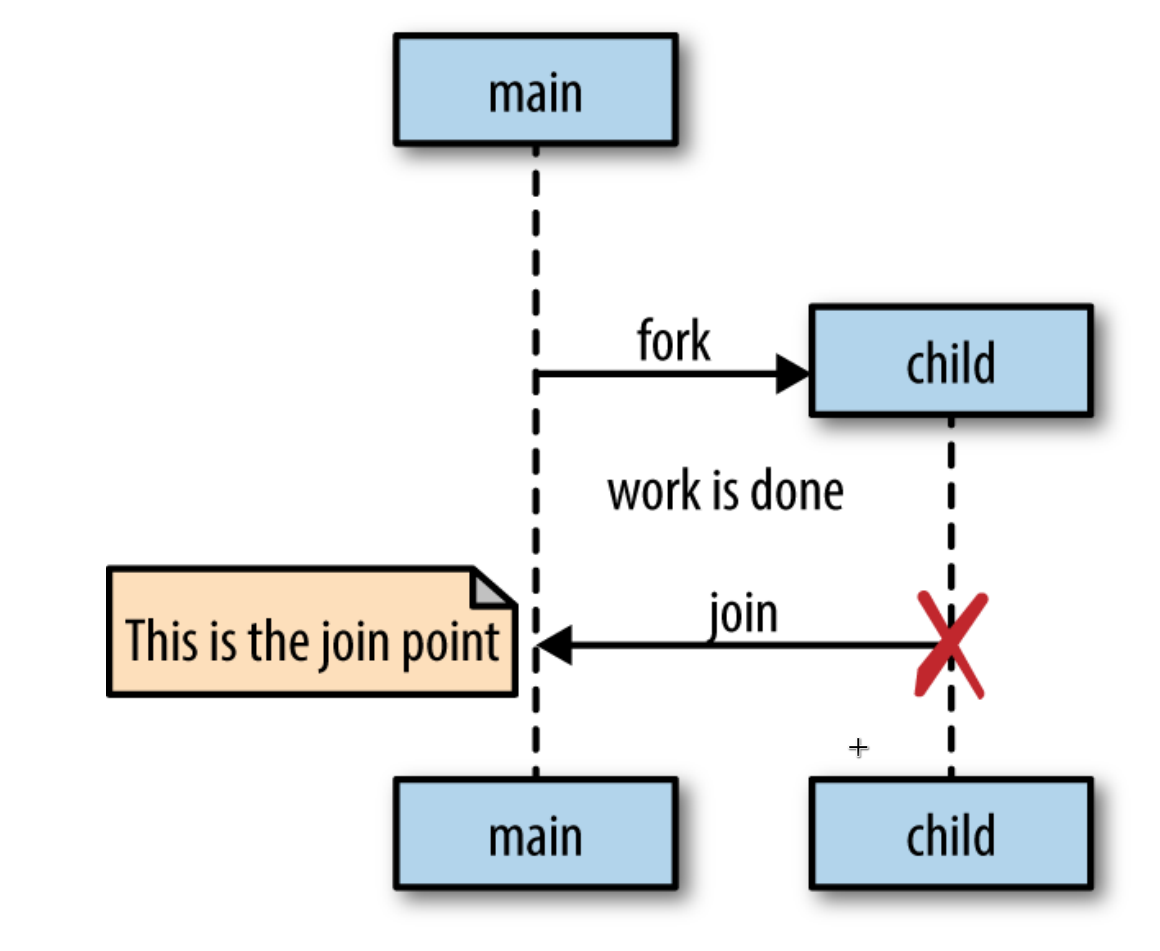
\includegraphics[width=\textwidth]{images/fork-join.png}
        \caption{分叉--汇合模型}
      \end{figure}
  \end{columns}
\end{frame}

\begin{frame}[fragile]{错误设置的汇合点}
\begin{lstlisting}[caption={不正确的汇合点引发竞态},label={wrong-join}]
sayHello := func() {
  fmt.Println("hello")
}
go sayHello()
// continue doing other things
\end{lstlisting}

    \alert{以上程序的输出结果是不确定的}。因为协程由 Go 运行时创建和调度,\code{sayHello}协程没能通过合适的汇合点和主协程进行汇合。因此,如果被调度之前主协程已退出,\code{sayHello}就无法获得执行的机会

    \begin{exampleblock}{温馨提示}
        \textbf{正确设置的汇点}能确保程序正确性并消除潜在的\alert{竞态} 
    \end{exampleblock}
\end{frame}

\begin{frame}[fragile]{纠正的汇合点}
为上述程序设置正确的汇合点,\texttt{sayHello}必须和主协程\textbf{同步},使自己能在主协程退出之前与其汇合,解决方案之一如\lstlistingname~\ref{lst-ok-join}

\begin{lstlisting}[caption={利用同步确保\texttt{sayHello}在主协程退出之前与其汇合},label=lst-ok-join]
var wg sync. WaitGroup
sayHello := func() {
  defer wg.Done()
  fmt.Println("hello")
}
wg.Add(1)
go sayHello()
wg.Wait()  // 汇合点

// 输出:
// hello    
\end{lstlisting}

\alert{可见,分叉---汇合模型下并发编程的正确性依赖于数据同步}
\end{frame}

\begin{frame}{数据同步方式}
\texttt{go}语言实现数据同步操作提供了两种方式
\begin{itemize}
    \item 传统地,\alert{共享内存型同步模式},常用元件分布在\texttt{sync}包
    \item \alert{基于顺序进程通信(CSP)}的消息传递实现数据同步,主要元件为通道\texttt{channel}及\texttt{select}语句
\end{itemize}
\end{frame}

    \section{sync包}
\begin{frame}{基本元件}
   \texttt{sync}包维护着用于同步底层内存访问的元件,包括
   \begin{itemize}
       \item \WaitGroup
       \item \Mutex 和 \RWMutex
       \item \Cond
       \item \Once
       \item \Pool
   \end{itemize} 
\end{frame}

    %\subsection{\WaitGroup}
\begin{frame}[fragile]{\WaitGroup}
   \textbf{用途}: 等待一批并发操作结束,\alert{操作的结果不是关心的重点或者能够通过其他途径收集} 

   \begin{columns}[t]
       \column{0.6\textwidth}
\begin{lstlisting}[xleftmargin=8pt]
var wg sync.WaitGroup

wg.Add(1)
go func() {
  defer wg.Done()
  fmt.Println("Alice sleeping...")
  time.Sleep(1)
}()

wg.Add(1)
go func() {
  defer wg.Done()
  fmt.Println("Bob sleeping...")
  time.Sleep(2)
}()
wg.Wait()
fmt.Println("Both are awaken.")
\end{lstlisting}

       \column{0.4\textwidth}
\begin{lstlisting}[firstnumber=last,xleftmargin=16pt]
// 输出:
// Bob sleeping...
// Alice sleeping...
// Both are awaken.
\end{lstlisting}
   \end{columns}
\end{frame}

\begin{frame}{\WaitGroup}
    \WaitGroup 可看作一个\alert{协程安全}的计数器

    \begin{itemize}
        \item 通过 \code{Add(x)}加上特定数\code{x}
        \item 通过 \code{Done()}使其减1
        \item \code{Wait()}使其一直阻塞直至计数器置零
    \end{itemize}

    \pause
    \begin{alertblock}{温馨提示}
        \code{Add()}需要在\WaitGroup 协调的协程之外(一般是主协程)调用,否则将引入\alert{竞态}
    \end{alertblock}
\end{frame}
    %\subsection{\Mutex 和\RWMutex }
\begin{frame}{基本介绍}
    \begin{itemize}
        \item \Mutex 是``Mutual Exclusion''的缩写
        \item \textbf{用途}: 保护程序的\alert{关键区域}---需要排他地存取共享资源的程序片段
        \item \Mutex 和\RWMutex 要求开发者必须以\alert{特定的方式}访问内存以保证数据的同步
    \end{itemize}
\end{frame}

\begin{frame}[fragile]{示例}
\begin{lstlisting}[caption={\Mutex 使用示例}]
var count int
var lock sync.Mutex

increment := func() {
  lock.Lock()
  defer lock.Unlock()
  count++
  fmt.Printf("Incrementing: %d\n", count)
}
decrement := func() {
  lock.Lock() // 请求对关键区域--count变量的存取
  defer lock.Unlock()  // 放弃对关键区域的排他存取权利
  count--
  fmt.Printf("Decrementing: %d\n", count)
}
\end{lstlisting}
\end{frame}

\begin{frame}[fragile]{示例(续)}
    \begin{columns}[t]
        \begin{column}{0.5\textwidth}
\begin{lstlisting}[caption={\Mutex 使用示例(续)},firstnumber=last,xleftmargin=8pt]
// Increment
var arithmetic sync.WaitGroup
for i := 0; i <= 2; i++ {
  arithmetic.Add(1)
  go func() {
    defer arithmetic.Done()
    increment()
  }()
}
// Decrement
for i := 0; i <= 2; i++ {
  arithmetic.Add(1)
  go func() {
    defer arithmetic.Done()
\end{lstlisting}
        \end{column}
        \begin{column}{0.5\textwidth}
\begin{lstlisting}[caption={\Mutex 使用示例(续)},firstnumber=last,xleftmargin=8pt]
    decrement()
  }()
}
arithmetic.Wait()
fmt.Println("Arithmetic complete.")

// 输出:
// Decrementing: -1
// Incrementing: 0
// Incrementing: 1
// Decrementing: 0
// Decrementing: -1
// Incrementing: 0
// Arithmetic complete.
\end{lstlisting}
        \end{column}
    \end{columns}
\end{frame}

\begin{frame}{温馨提示}
    \begin{itemize}
        \item 锁\texttt{m}的\texttt{Lock()}调用之后应有配对的\texttt{defer m.UnLock()}语句
        \item \alert{进出关键区域的代价是昂贵的}
    \end{itemize}    
\end{frame}

\begin{frame}{读写锁\RWMutex }
    \alert{在写锁未被锁定之前},读写锁能够满足任意共存的读锁请求

    示例代码参见\href{https://github.com/sammyne/concurrency-in-go/blob/master/chapter03/sync.pkg/mutex/rwlock.go}{\Mutex 和\RWMutex 性能对比},具体结果如下图所示,\alert{可见,性能替身没有想象中的那么明显}

    \begin{figure}
        \centering
        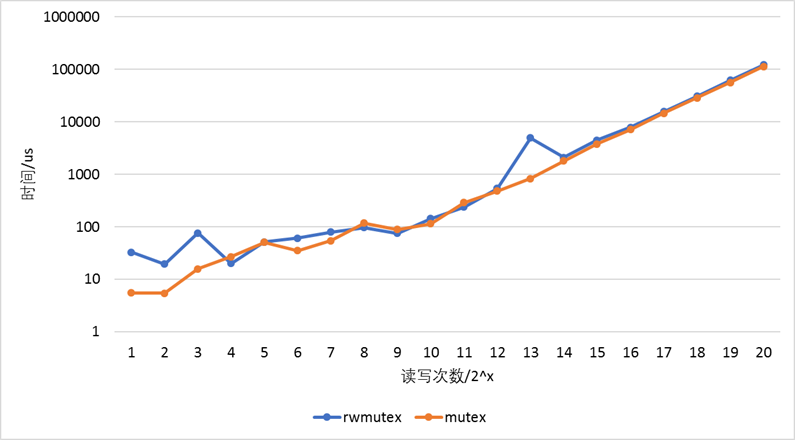
\includegraphics[width=0.7\textwidth]{images/rwmutex-vs-mutex.png}
        \caption{\Mutex 和\RWMutex 性能对比结果}
    \end{figure}
\end{frame}

\iffalse
\begin{frame}{读写锁\RWMutex }
    \alert{在写锁未被锁定之前},读写锁能够满足任意共存的读锁请求

    示例代码参见\href{https://github.com/sammyne/concurrency-in-go/blob/master/chapter03/sync.pkg/mutex/rwlock.go}{\Mutex 和\RWMutex 性能对比}

    程序的输出结果类似
    \begin{columns}
        \column{0.5\textwidth}
            \begin{table}
                \centering
                \caption{\Mutex 和\RWMutex 性能对比}
                \begin{tabular}{lll}
                    \hline
                    Readers  &RWMutex       &Mutex  \\
                    \hline
                    1        &32.87µs       &5.541µs \\
                    2        &19.603µs      &5.439µs \\
                    4        &76.62µs       &15.886µs \\
                    8        &20.201µs      &26.892µs \\
                    16       &51.558µs      &50.657µs \\
                    32       &61.313µs      &34.999µs \\
                    \hline
                \end{tabular}
            \end{table}

        \column{0.5\textwidth}
            \begin{table}
                \centering
                \caption{\Mutex 和\RWMutex 性能对比(续)}
                \begin{tabular}{lll}
                    \hline
                    Readers  &RWMutex       &Mutex  \\
                    \hline
                    64       &79.628µs      &54.763µs \\
                    128      &96.749µs      &118.701µs \\
                    256      &75.414µs      &89.375µs \\
                    512      &142.882µs     &114.705µs \\
                    1024     &239.471µs     &289.861µs \\
                    2048     &540.809µs     &479.173µs \\ 
                    \hline
                \end{tabular}
            \end{table}
    \end{columns}
\end{frame}

\begin{frame}{读写锁\RWMutex }
            \begin{table}[htbp!]
                \caption{\Mutex 和\RWMutex 性能对比(续)}
                \begin{tabular}{lll}
                    \hline
                    Readers  &RWMutex       &Mutex  \\
                    \hline
                    2048     &540.809µs     &479.173µs \\ 
                    4096     &4.982512ms    &827.095µs \\
                    8192     &2.09599ms     &1.790277ms \\
                    16384    &4.47045ms     &3.820926ms \\
                    32768    &7.911863ms    &7.163938ms \\
                    65536    &15.689641ms   &14.66057ms \\
                    131072   &31.016011ms   &28.674835ms \\
                    262144   &62.493129ms   &56.609731ms \\
                    524288   &121.927969ms  &113.786247ms \\   
                    \hline
                \end{tabular}
            \end{table} 
\end{frame}
\fi

    \iffalse
    \section{Section 1}
    \begin{frame}{Simple frame}
        This is a simple frame.
    \end{frame}

    \begin{frame}[plain]{Plain frame}
        This is a frame with plain style and it is numbered.
    \end{frame}
    
    \begin{frame}[t]
        This frame has an empty title and is aligned to top.
    \end{frame}
    
    \begin{frame}[noframenumbering]{No frame numbering}
        This frame is not numbered and is citing reference \cite{knuth74}.
    \end{frame}
    
    \begin{frame}{Typesetting and Math}
        The packages \texttt{inputenc} and \texttt{FiraSans}\footnote{\url{https://fonts.google.com/specimen/Fira+Sans}}\textsuperscript{,}\footnote{\url{http://mozilla.github.io/Fira/}} are used to properly set the main fonts.
        \vfill
        This theme provides styling commands to typeset \emph{emphasized}, \alert{alerted}, \textbf{bold}, \textcolor{example}{example text}, \dots
        \vfill
        \texttt{FiraSans} also provides support for mathematical symbols:
        \begin{equation*}
            e^{i\pi} + 1 = 0.
        \end{equation*}
    \end{frame}

    \section{Section 2}
    \begin{frame}{Blocks}
        \begin{block}{Block}
            Text.
        \end{block}
        \pause
        \begin{alertblock}{Alert block}
            Alert \alert{text}.
        \end{alertblock}
        \pause
        \begin{exampleblock}{Example block}
            Example \textcolor{example}{text}.
        \end{exampleblock}
    \end{frame}
    
    \begin{frame}{Lists}
        \begin{columns}[t, onlytextwidth]
            \column{0.33\textwidth}
                Items:
                \begin{itemize}
                    \item Item 1
                    \begin{itemize}
                        \item Subitem 1.1
                        \item Subitem 1.2
                    \end{itemize}
                    \item Item 2
                    \item Item 3
                \end{itemize}
            
            \column{0.33\textwidth}
                Enumerations:
                \begin{enumerate}
                    \item First
                    \item Second
                    \begin{enumerate}
                        \item Sub-first
                        \item Sub-second
                    \end{enumerate}
                    \item Third
                \end{enumerate}
            
            \column{0.33\textwidth}
                Descriptions:
                \begin{description}
                    \item[First] Yes.
                    \item[Second] No.
                \end{description}
        \end{columns}
    \end{frame}
\setbeamertemplate{caption}[numbered]
    \begin{frame}{Figures and Tables}
        \begin{columns}
            \column{0.4\textwidth}
                \begin{figure}
                    \centering
                    
\includegraphics{focuslogo.pdf}
                    \caption{Figure caption.}
                    \label{fig:focuslogo}
                \end{figure}
                
            \column{0.6\textwidth}
                \begin{table}
                    \centering
                    \begin{tabular}{rcc}
                         & Heading 1 & Heading 2 \\\hline
                        Row 1 & \(v_{11}\) & \(v_{12}\) \\
                        Row 2 & \(v_{21}\) & \(v_{22}\) \\
                        Row 3 & \(v_{31}\) & \(v_{32}\) \\
                    \end{tabular}
                    \caption{Table caption.}
                    \label{tab:demo}
                \end{table}
        \end{columns}
    \end{frame}
    
    \begin{frame}[focus]
        Thanks for using \textbf{Focus}!
    \end{frame}
    
    \appendix
    \begin{frame}{References}
        \nocite{*}
        \bibliography{demo_bibliography}
        \bibliographystyle{plain}
    \end{frame}
    
    \begin{frame}{Backup frame}
        \usebeamercolor[fg]{normal text}
        This is a backup frame, useful to include additional material for questions from the audience.
        \vfill
        The package \texttt{appendixnumberbeamer} is used not to number appendix frames.
    \end{frame}
    \fi
\end{document}
